\changecolours{ScoutRed}
\section{Taxonomia NoSQL \& Prática Hands-On}

% ------------------------------------------------------------------------------
\twocolframe[title={Os 4 Modelos NoSQL \& Bancos Vetoriais},leftcol=7cm,rightcol=7cm]{%
  \alert{Modelos Orientados a Agregados}\par
  \itemseps[topsepi=1.5mm,itemsepi=2.5mm,labelsep=2mm,leftmargini=4mm]
  \begin{itemize}
    \item \textbf{Chave-Valor (Redis, DynamoDB):} Dicionários gigantes em memória. Complexidade $O(1)$. Foco em cache e latência (\textbf{PA/EL} ou \textbf{PC/EL}).
    \item \textbf{Documentos (MongoDB, Couchbase):} JSON/BSON com esquemas flexíveis e aninhamento. Foco em aplicações web e catálogos (\textbf{PC/EC}).
    \item \textbf{Família de Colunas (Cassandra, ScyllaDB):} Colunas esparsas distribuídas em anel \textit{masterless}. Escrita massiva (\textbf{PA/EL}).
  \end{itemize}
}{%
  \alert{Grafos \& Bancos Vetoriais}\par
  \itemseps[topsepi=1.5mm,itemsepi=2.5mm,labelsep=2mm,leftmargini=4mm]
  \begin{itemize}
    \item \textbf{Orientados a Grafos (Neo4j):} Foco na riqueza de relacionamentos e travessia rápida de caminhos (\textbf{PC/EC}).
    \item \textbf{Bancos Vetoriais (ChromaDB, Pinecone):} Vetores de alta dimensão (*embeddings*) para busca semântica e IA Generativa (RAG).
  \end{itemize}
}

% ------------------------------------------------------------------------------
\begin{frame}{Taxonomia NoSQL na Matriz CAP / PACELC}
  \vspace{-0.3cm}
  \makebox[\linewidth][c]{%
    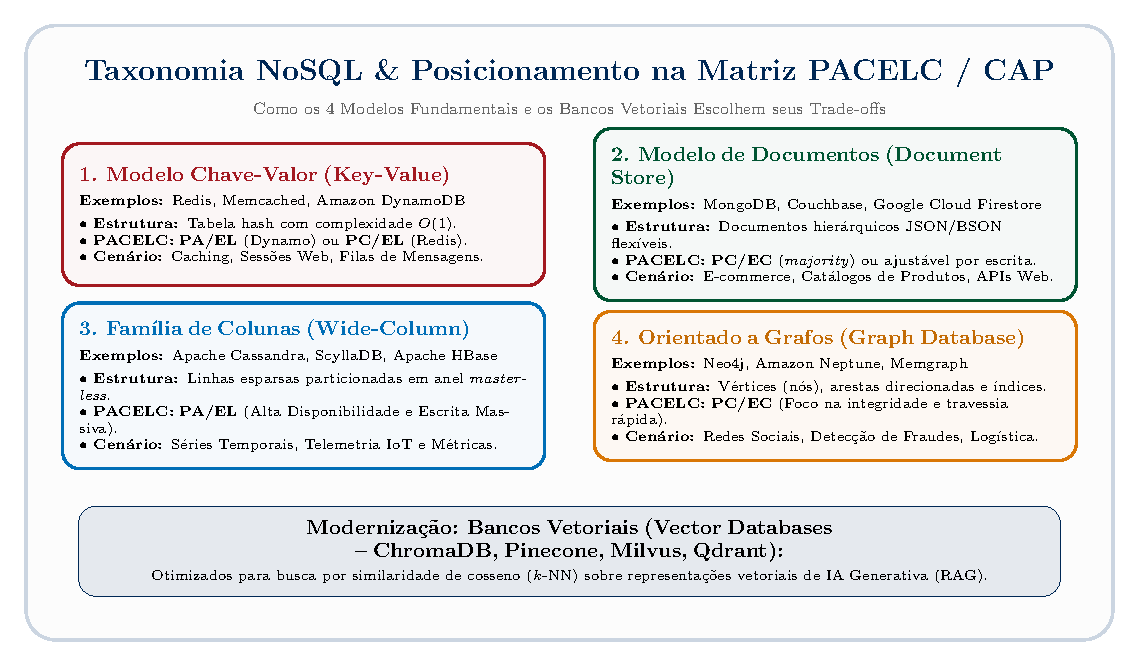
\includegraphics[width=14.0cm,height=4.8cm,keepaspectratio]{figuras/fig_taxonomia_4_modelos.pdf}%
  }\par
  \vspace{0.15cm}
  \centering
  {\footnotesize \textbf{Síntese Arquitetural:} \textcolor{ScoutRed}{Cada modelo NoSQL foi desenhado para resolver um tipo específico de acesso e trade-off.}}
\end{frame}

% ------------------------------------------------------------------------------
\begin{frame}[fragile]{MongoDB Prático: Níveis de Garantia de Escrita (Write Concern)}
\vspace{-0.2cm}
\alert{Ajustando o Teorema PACELC diretamente no código de aplicação:}\par
\vspace{0.1cm}
\begin{lstlisting}
// 1. Alta Performance / Baixa Latencia (Modo PA/EL):
db.sensores.insertOne(
  { sensor: "TAU-01", temp: 31.2 },
  { writeConcern: { w: 1, wtimeout: 1000 } }
);

// 2. Alta Seguranca e Consistencia Financeira (Modo PC/EC):
db.transferencias.insertOne(
  { de: "CTA-100", para: "CTA-200", valor: 1500.00 },
  { writeConcern: { w: "majority", j: true, wtimeout: 5000 } }
);
\end{lstlisting}
\vspace{-0.1cm}
\centering
{\scriptsize \textbf{Nota de Engenharia:} O parâmetro \texttt{w: "majority"} impede que alterações sejam revertidas por eleições de novo líder.}
\end{frame}

% ------------------------------------------------------------------------------
\begin{frame}[fragile]{MongoDB Prático: Níveis de Isolamento de Leitura (Read Concern)}
\vspace{-0.2cm}
\alert{Controlando se sua consulta pode ou não ler dados defasados (Stale Reads):}\par
\vspace{0.1cm}
\begin{lstlisting}
// 1. Leitura Local (Rapida, mas com risco de Stale Read):
db.pedidos.find({ status: "pendente" }).readConcern("local");

// 2. Leitura com Quorum Garantido (Majority Read Concern):
db.pedidos.find({ id_pedido: "PED-2026-09" }).readConcern("majority");

// 3. Leitura Linearizavel (Linearizable):
db.contas.find({ id_cliente: 42 }).readConcern("linearizable");
\end{lstlisting}
\end{frame}

% ------------------------------------------------------------------------------
\twocolframe[title={Roteiro do Laboratório Hands-On no Terminal},leftcol=7cm,rightcol=7cm]{%
  \alert{O Script Didático da Aula}\par
  \itemseps[topsepi=2mm,itemsepi=3mm,labelsep=2mm,leftmargini=4mm]
  \begin{itemize}
    \item Desenvolvido especificamente para esta aula: \texttt{demonstracao\_aula02.py}.
    \item Simula um cluster de 3 nós com injeção de rompimento de rede em tempo real.
    \item Demonstra na prática:
      \begin{itemize}
        \item Bloqueio de escritas sem quórum (CP);
        \item Escrita local e leitura defasada (AP);
        \item Reconciliação via \textit{Last-Write-Wins}.
      \end{itemize}
  \end{itemize}
}{%
  \alert{Como Executar no Laboratório}\par
  \itemseps[topsepi=2mm,itemsepi=3mm,labelsep=2mm,leftmargini=4mm]
  \begin{itemize}
    \item Abra o terminal na pasta da aula e execute:
    \item \texttt{python3 codigo/demonstracao\_aula02.py}
    \item Navegue pelo menu interativo (opções 1 a 5).
    \item Também disponível como Jupyter Notebook interativo:
    \item \texttt{codigo/demonstracao\_aula02.ipynb}
  \end{itemize}
}

% ------------------------------------------------------------------------------
\twocolframe[title={Próximo Encontro \& Atividades de Fixação},leftcol=7cm,rightcol=7cm]{%
  \alert{Sábado Letivo (10/10/2026) -- Aula 03}\par
  \itemseps[topsepi=2mm,itemsepi=3mm,labelsep=2mm,leftmargini=4mm]
  \begin{itemize}
    \item \textbf{Atenção:} Conforme o cronograma pedagógico, sábado letivo \textbf{não tem conteúdo novo}.
    \item \textbf{Oficina Prática de DevOps:} Orquestração com Docker e Docker Compose para subir instâncias de Redis e MongoDB em segundos.
    \item Resolução assistida da Lista 1 no laboratório.
  \end{itemize}
}{%
  \alert{Lista de Exercícios 1 (Bloco 2)}\par
  \itemseps[topsepi=2mm,itemsepi=3mm,labelsep=2mm,leftmargini=4mm]
  \begin{itemize}
    \item Responder às questões 7 a 12 no \texttt{README.md} da Aula 02:
      \begin{itemize}
        \item Análise de partição em 3 e 4 nós;
        \item Trade-offs de Latência vs Consistência no PACELC;
        \item Comparação de cenários do mundo real (PIX vs TikTok);
        \item Uso de Write Concern no MongoDB.
      \end{itemize}
  \end{itemize}
}
